\subsubsection{\qqZZ~ Modelling}
\label{sec:redbkgd}

The \qqZZ~ background is generated at NLO, while the fully differential cross section has been computed at 
NNLO~\cite{Grazzini2015407}, but are not yet available in a partonic level event generator. Therefore NNLO/NLO 
$k$-factors for the \qqZZ~background process are applied to the {\sc powheg} sample. The inclusive cross 
sections obtained using the same PDF and renormalization and factorization scales as the {\sc powheg} sample
at LO, NLO, and NNLO are shown in Table~\ref{tab:qqZZXS}. The NNLO/NLO $k$-factors are applied in the analysis
differentally as a function of $m(\cPZ\cPZ)$. 

Additional NLO electroweak corrections which depend on the initial state quark flavor and kinematics
are also applied to the \qqZZ~ background process in the region $m(\cPZ \cPZ)>2m(\cPZ)$ where the 
corrections have been computed. The differential QCD and electroweak $k$-factors can be seen in 
Figure~\ref{fig:qqZZKfactor}.

\begin{table}[h]
    \centering
    \begin{tabular}{|l|c|c|} 
\hline %----------------------------------------------------------------
QCD Order  & $\sigma_{2\ell2\ell^{\prime}} (\mathrm{fb})$  & $\sigma_{4\ell} (\mathrm{fb})$  \\
\hline %----------------------------------------------------------------
LO    & 218.5$^{+16\%}_{-15\%}$ & 98.4$^{+13\%}_{-13\%}$ \\
NLO   & 290.7$^{+5\%}_{-8\%}$   & 129.5$^{+4\%}_{-6\%}$ \\
NNLO  & 324.0$^{+2\%}_{-3\%}$   & 141.2$^{+2\%}_{-2\%}$ \\
\hline %----------------------------------------------------------------
    \end{tabular}
    \caption{Cross sections for \qqZZ~ production at 13 \TeV}
    \label{tab:qqZZXS}
\end{table}

%=======
\begin{figure}[!htb]
\vspace*{0.3cm}
\begin{center}
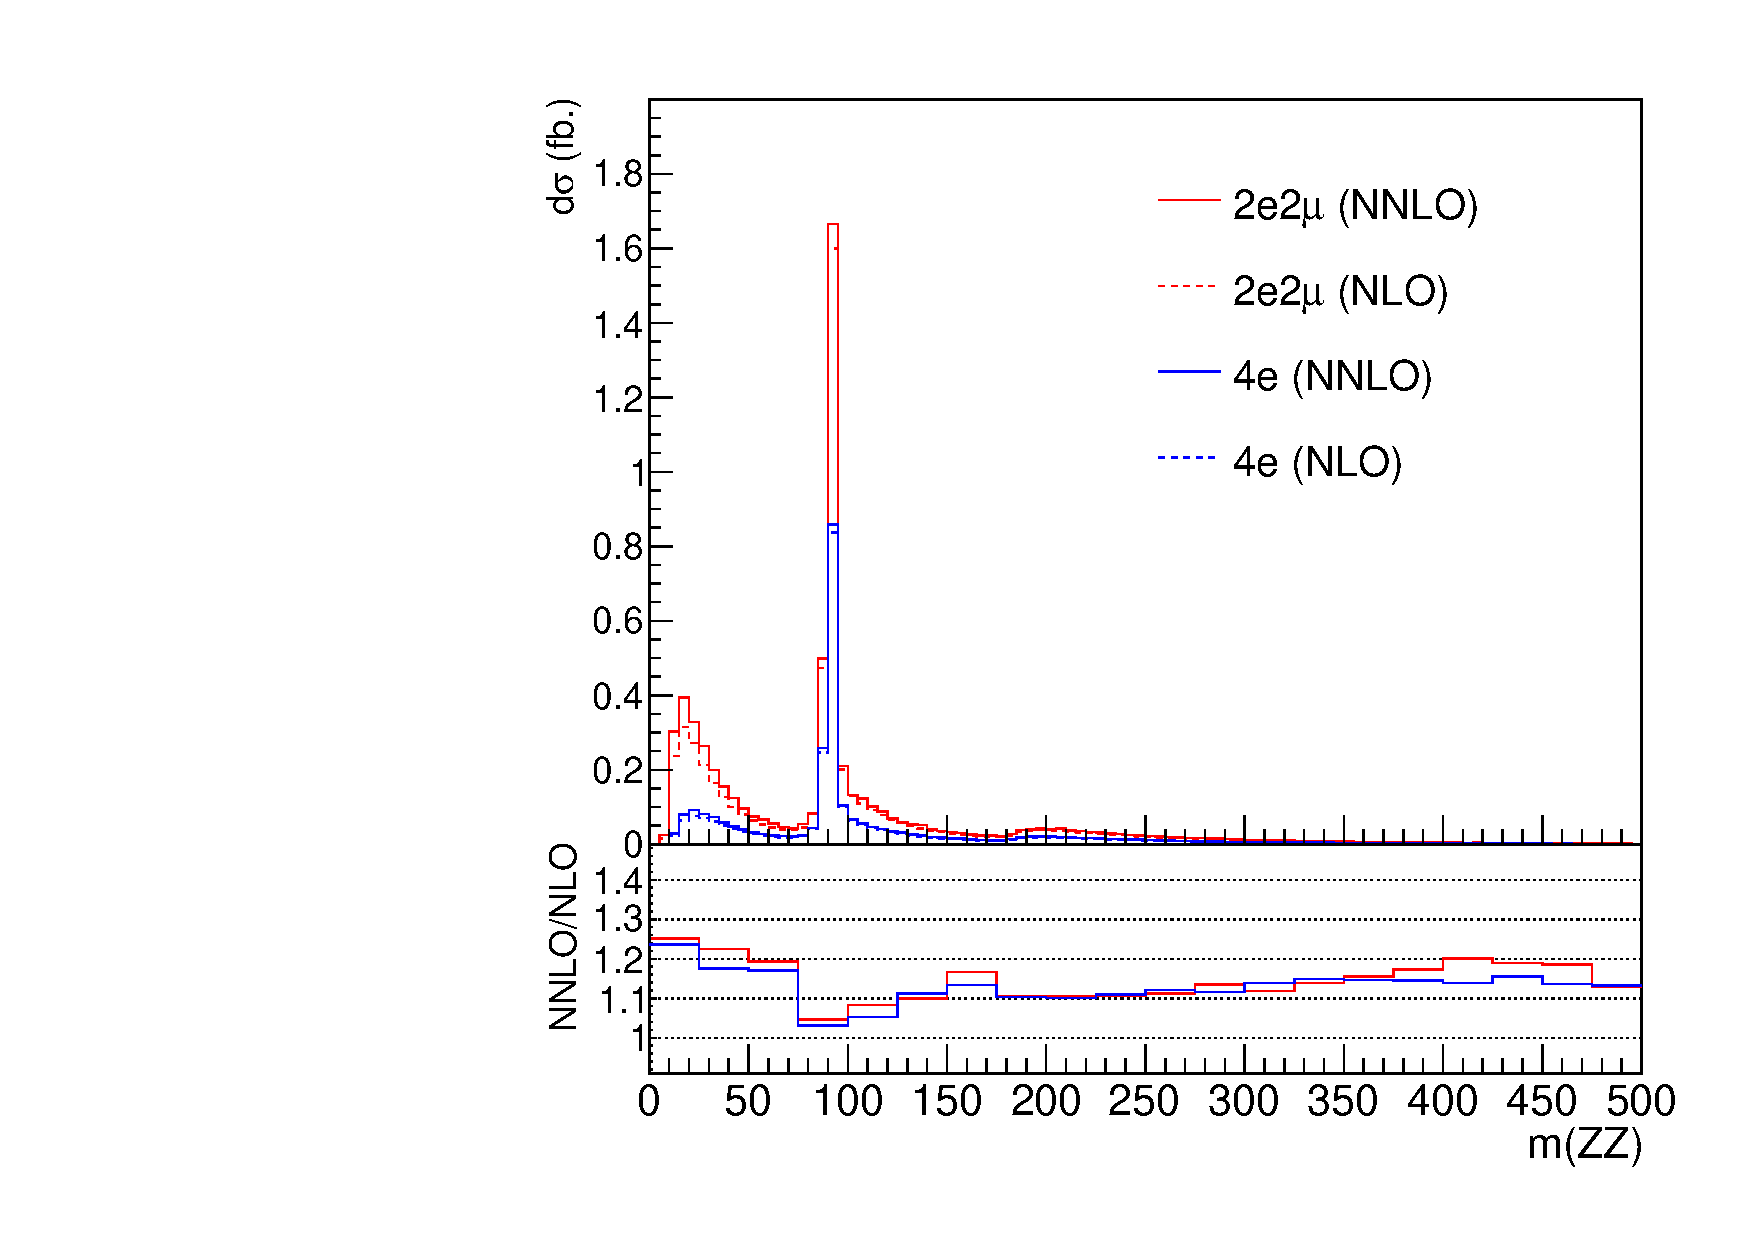
\includegraphics[width=0.48\textwidth]{Figures/IrrBkg/Kfactor_qqZZ_mZZ.pdf}
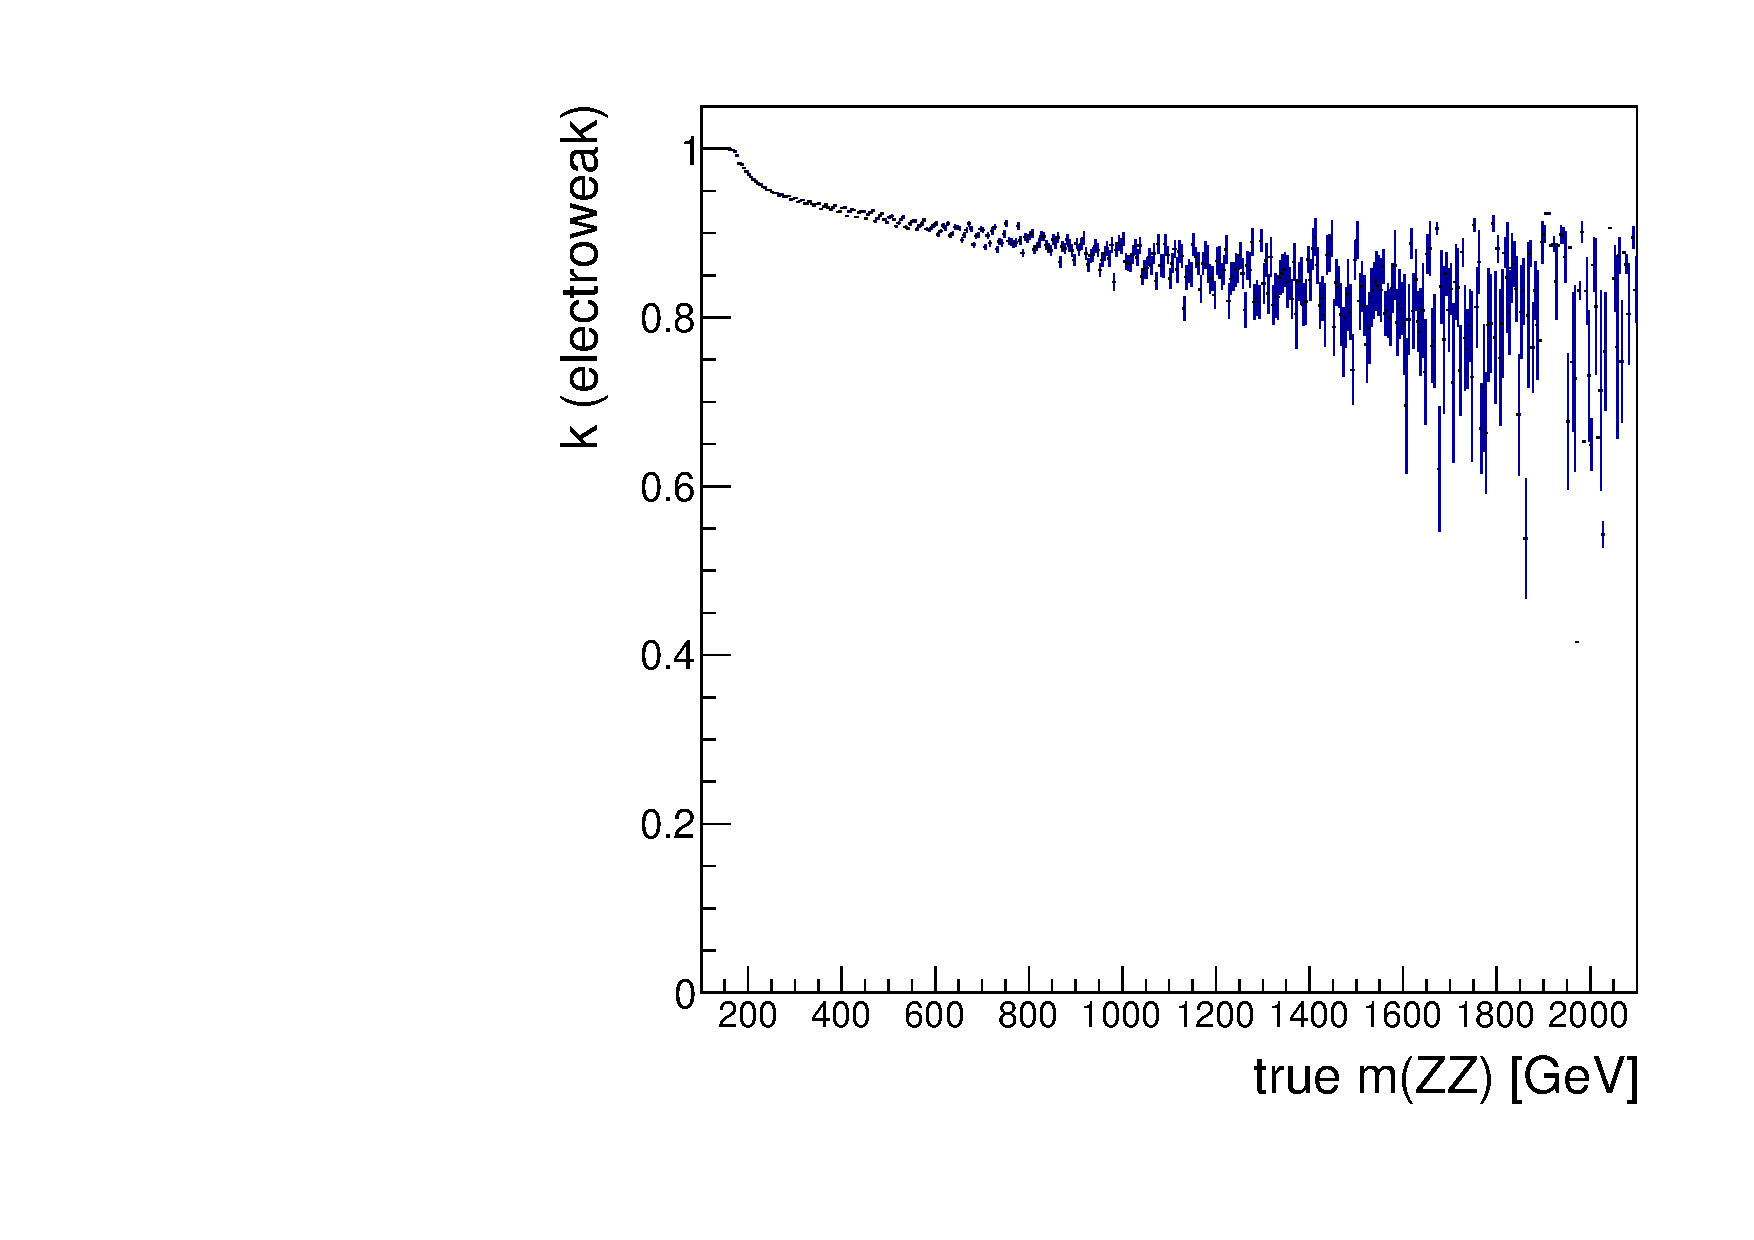
\includegraphics[width=0.48\textwidth]{Figures/IrrBkg/K_ewk_qqZZ.pdf} 
\caption{Left: NNLO/NLO QCD K factor for the \qqZZ~ background as a function of $m(ZZ)$ for the $4\ell$ and $2\ell2\ell^{\prime}$ final states. Right: NLO/NLO electroweak K factor for the \qqZZ~ background as a function of $m(ZZ)$.
\label{fig:qqZZKfactor}}
\end{center}
\end{figure}


\subsubsection{\ggZZ~ Modelling}

Event simulation for the $\ggZZ$ background is done at LO with the generator \MCFM~7.0~\cite{MCFM,Campbell:2011bn,Campbell:2013una}.
Although no exact calculation exists beyond the LO for the $\ggZZ$ background, 
it has been recently shown~\cite{Bonvini:1304.3053} 
that the soft collinear approximation is able to describe the background cross section and the 
interference term at NNLO\@. Further calculations also show that the K factors are very similar at NLO for the signal 
and background~\cite{Melnikov:2015laa} and at NNLO for the signal and interference terms~\cite{Li:2015jva}. Therefore, the same K factor 
is used for the signal and background~\cite{Passarino:1312.2397v1}. The NNLO K factor for the signal is obtained as a function of $\mllll$ 
using the \textsc{hnnlo}~v2 Monte Carlo program~\cite{Catani:2007vq,Grazzini:2008tf,Grazzini:2013mca} by calculating the NNLO and LO 
$\Pg\Pg\to\PH\to2\ell2\ell^\prime$ cross sections at the small $\PH$ boson decay width of $4.07$~\MeV and taking their ratios. The NNLO as 
well as the NLO K factors and the cross sections from which they are derived are illustrated in Figure~\ref{fig:ggHZZXsecKfactor}, 
along with the NNLO, NLO and LO cross sections at the SM $\PH$ boson decay width~\cite{Heinemeyer:2013tqa}.
 
\begin{figure}[!htb]
\centering
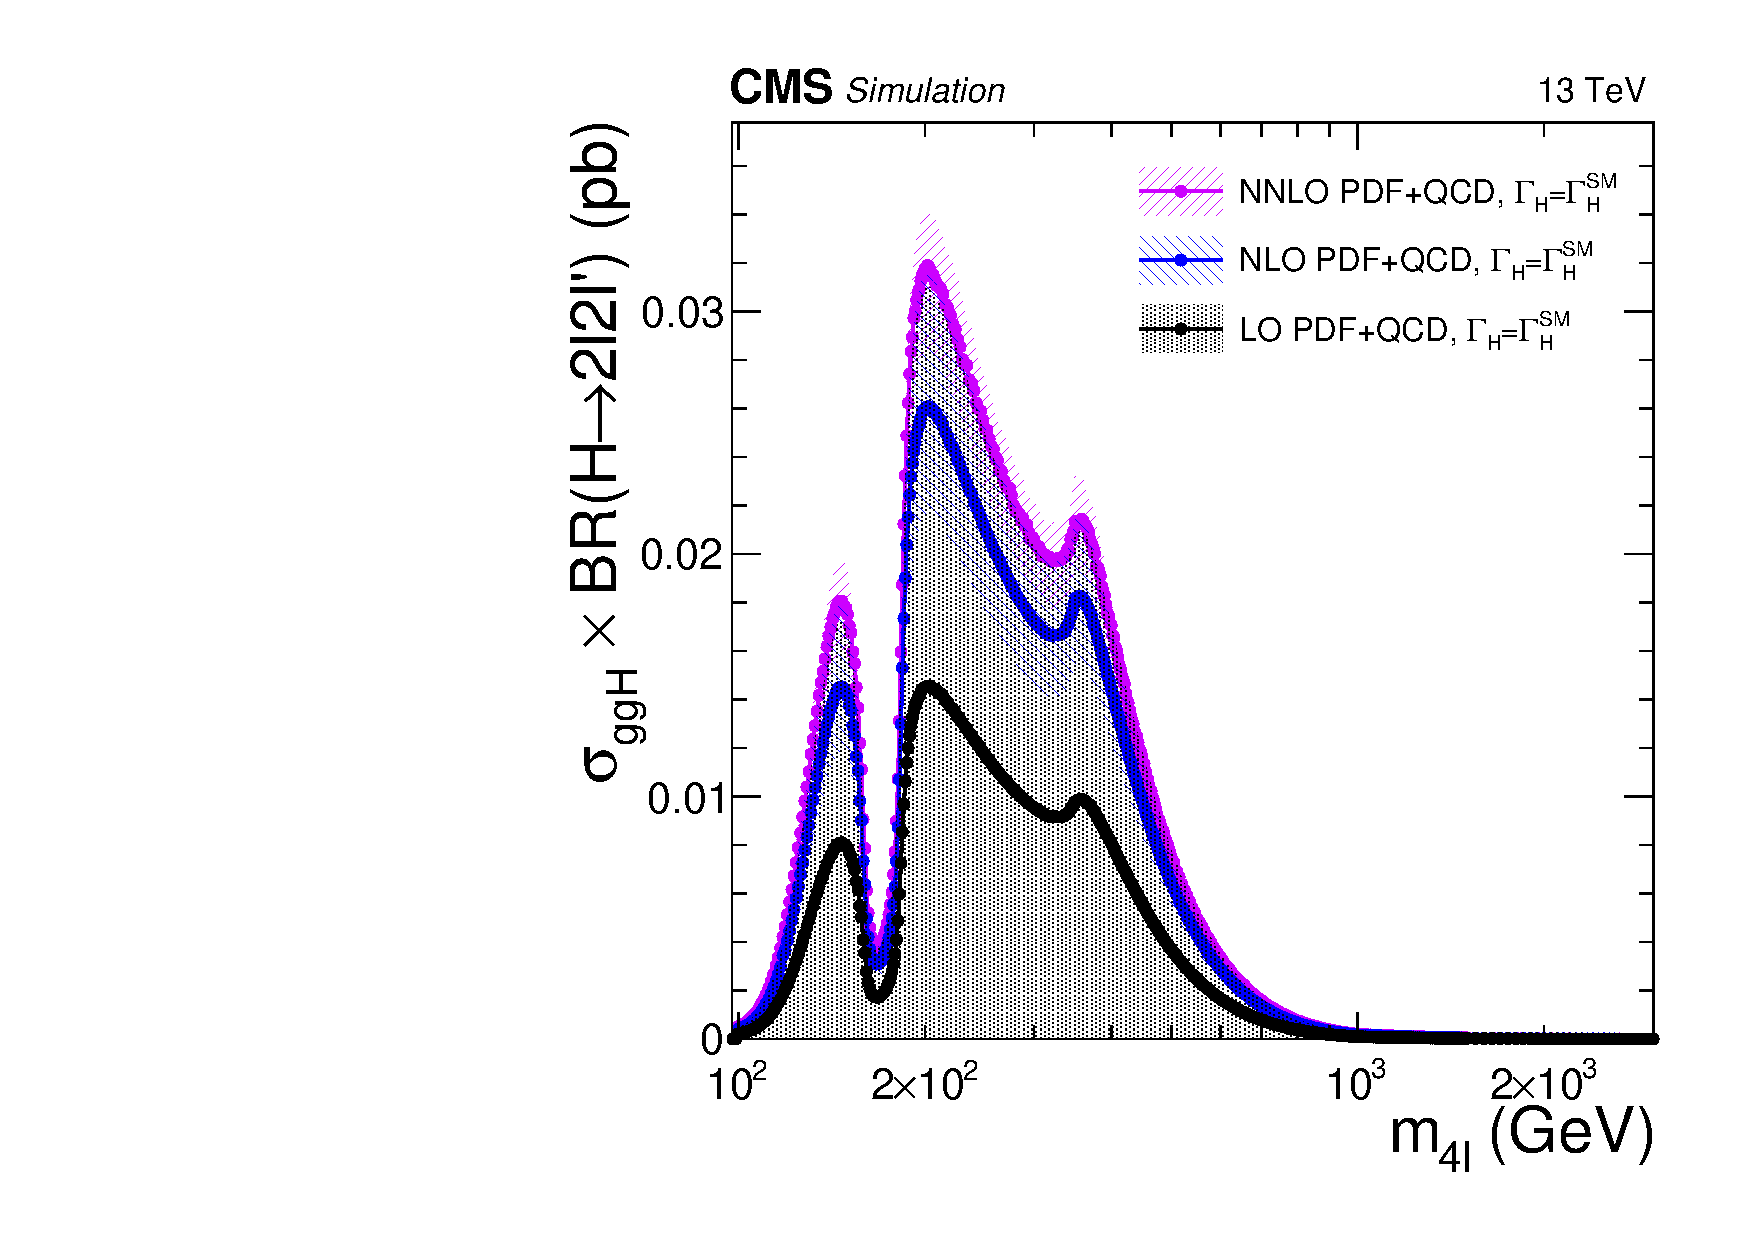
\includegraphics[width=0.48\linewidth]{Figures/IrrBkg/cCompare_hnnlo_ggHZZ2l2l_xsec.pdf}
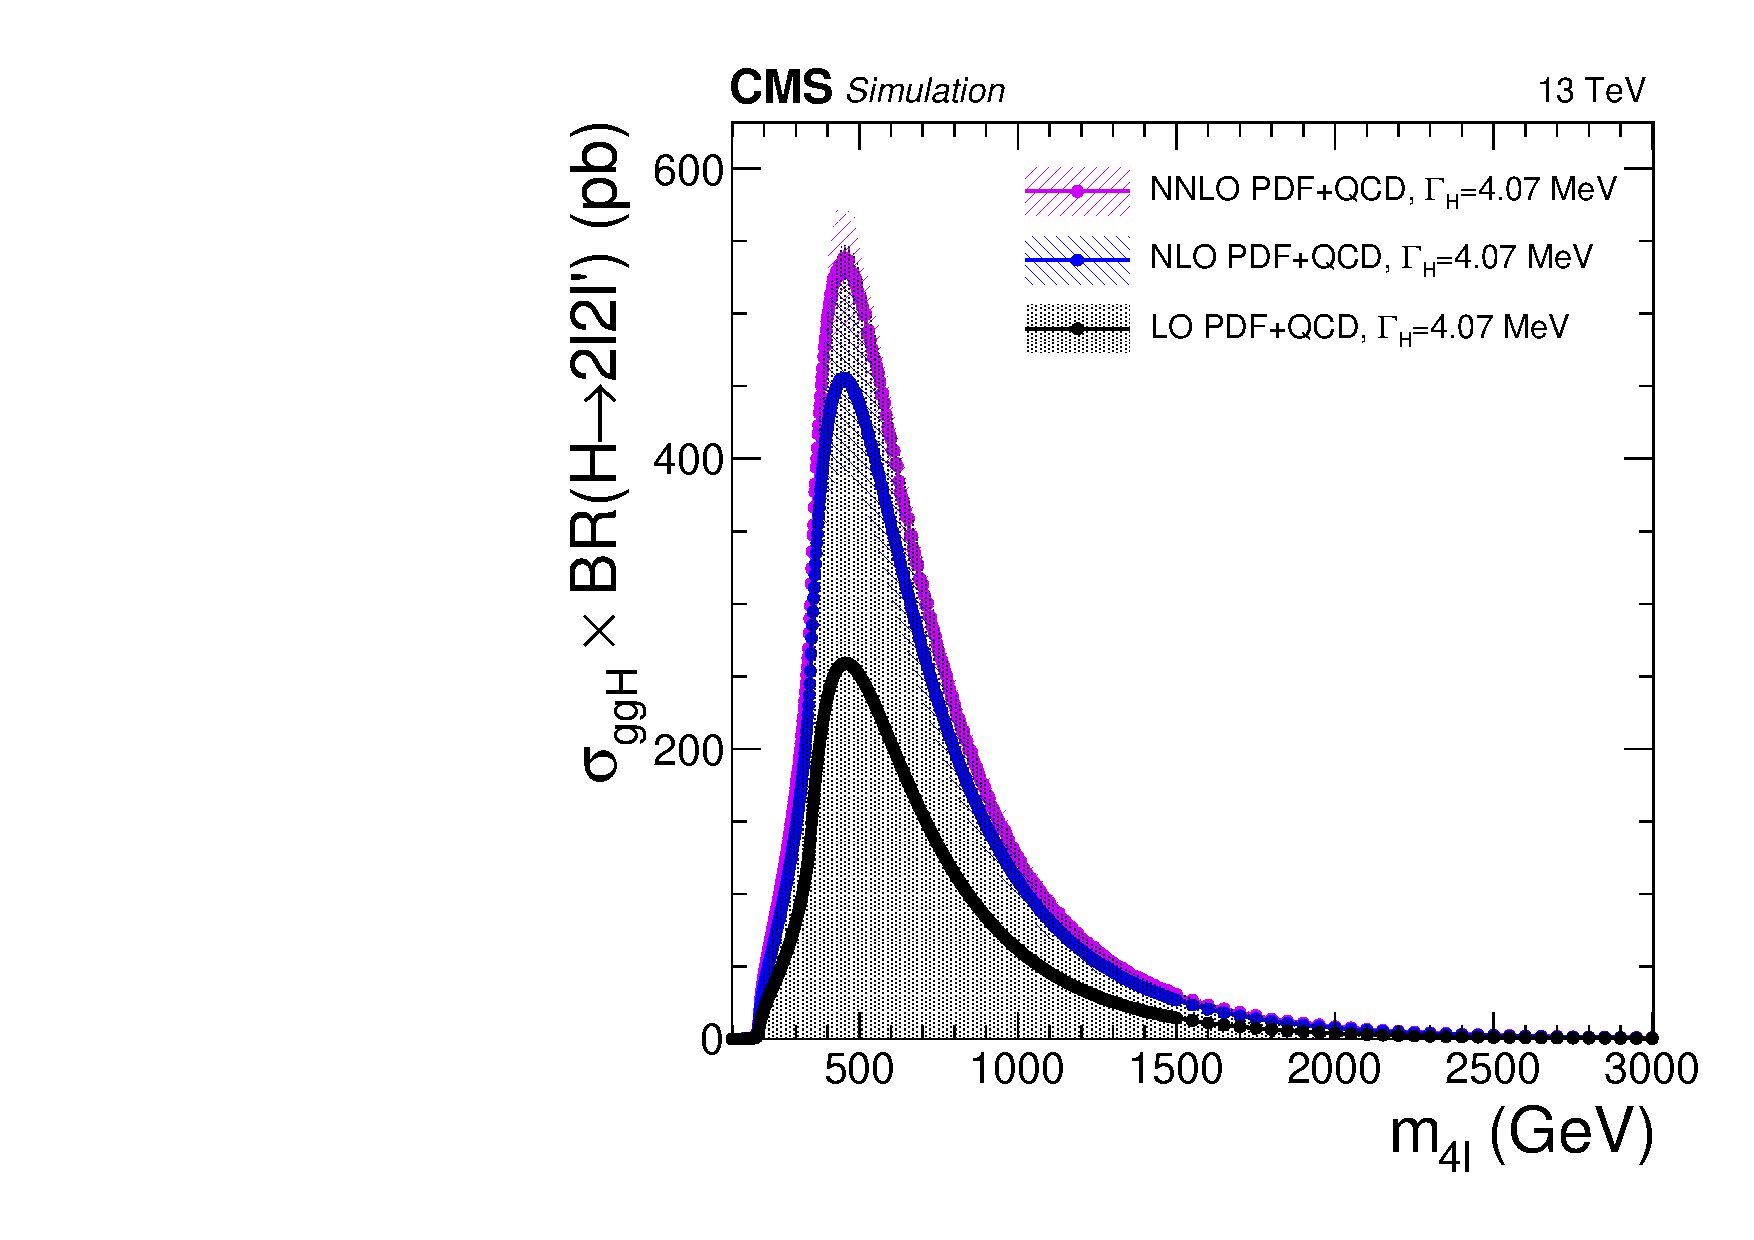
\includegraphics[width=0.48\linewidth]{Figures/IrrBkg/cCompare_hnnlo_ggHZZ2l2l_narrowwidth_xsec.pdf}\\
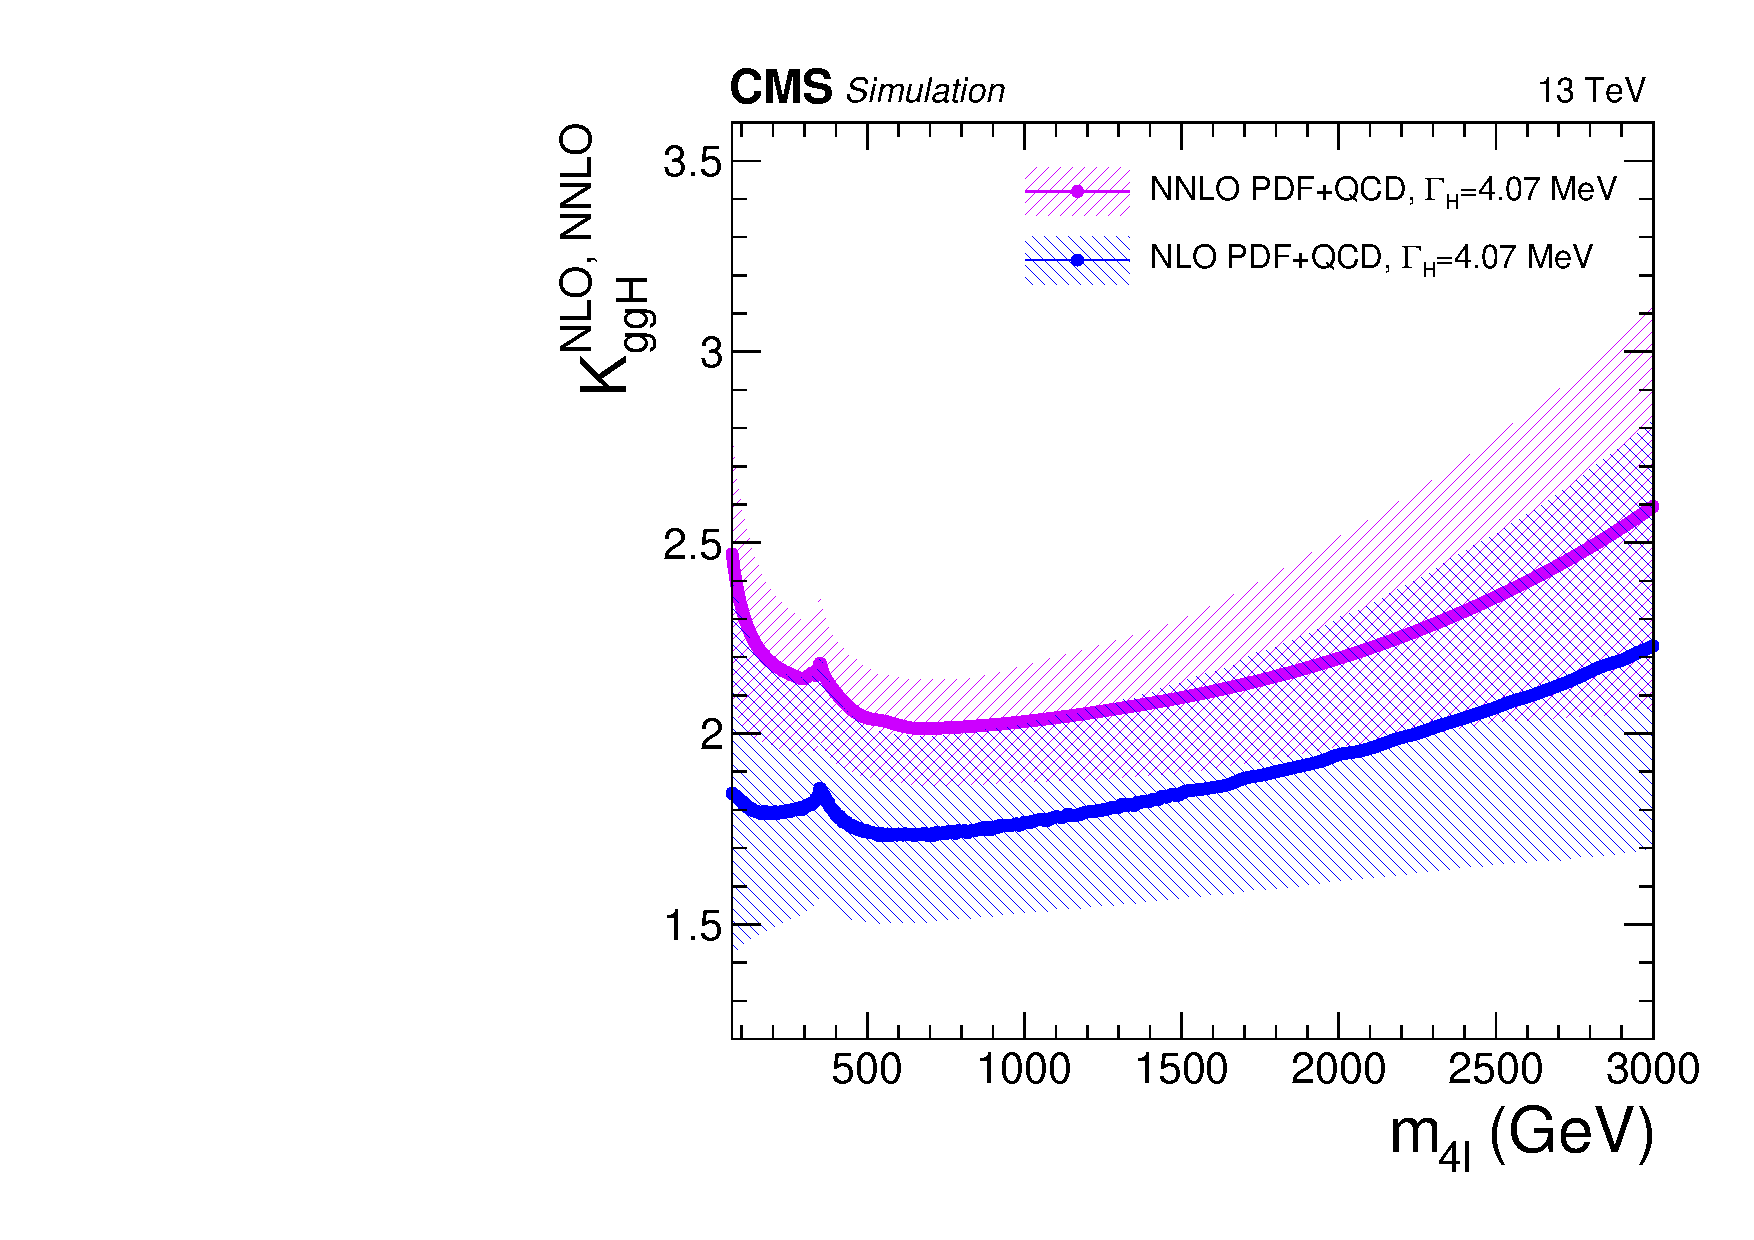
\includegraphics[width=0.48\linewidth]{Figures/IrrBkg/cCompare_hnnlo_ggHZZ2l2l_narrowwidth_kfactor.pdf}
\caption{$\Pg\Pg\to\PH\to2\ell2\ell^\prime$ cross sections at NNLO, NLO and LO at each $\PH$ boson pole mass using the SM $\PH$ boson decay width  (top left) or at the fixed and small decay width of $4.07$~MeV (top right). The cross sections using the fixed value are used to obtain the K factor for both the signal and the continuum background contributions as a function of $\mllll$ (bottom).
}
\label{fig:ggHZZXsecKfactor}
\end{figure}

